\documentclass[tikz,border=5pt]{standalone}
\usepackage{tikz}
\usepackage{pgfplots}
\pgfplotsset{compat=1.18}

\begin{document}
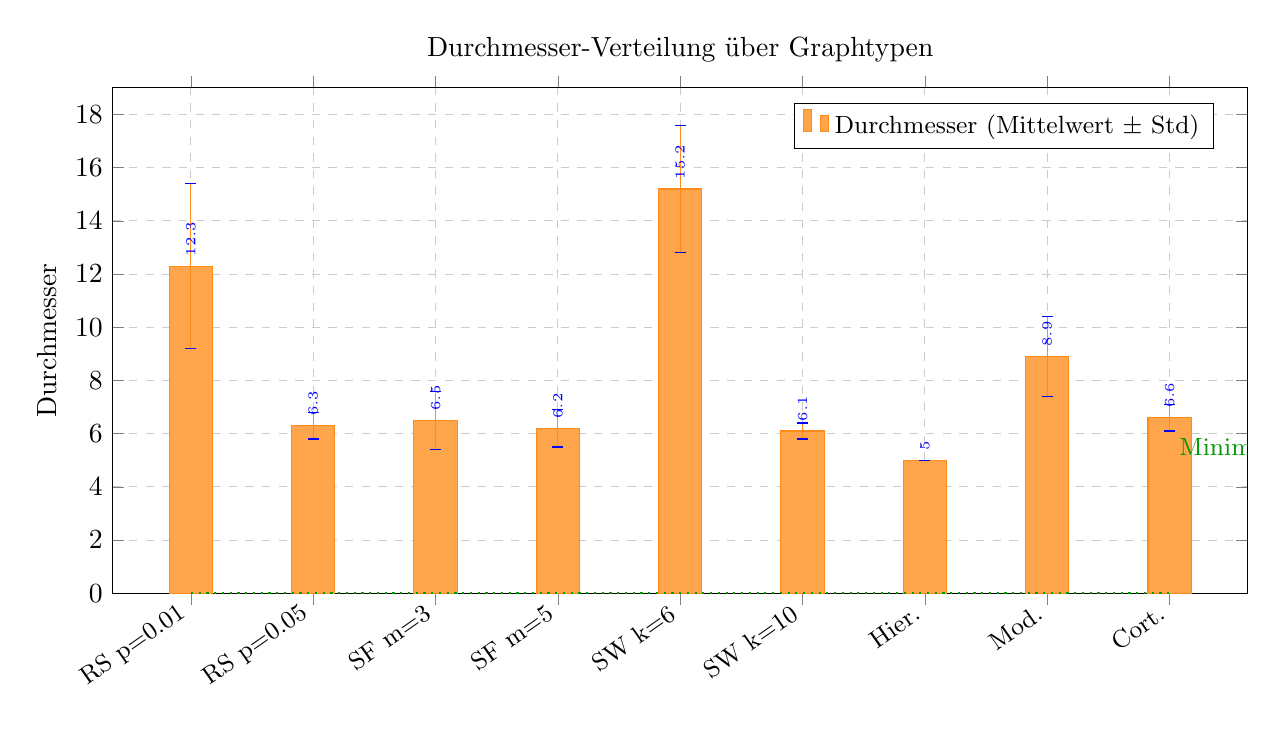
\begin{tikzpicture}
\begin{axis}[
    width=16cm,
    height=8cm,
    ybar,
    bar width=0.55cm,
    enlarge x limits=0.08,
    ylabel={Durchmesser},
    title={Durchmesser-Verteilung \"{u}ber Graphtypen},
    symbolic x coords={
        RS p=0.01,
        RS p=0.05,
        SF m=3,
        SF m=5,
        SW k=6,
        SW k=10,
        Hier.,
        Mod.,
        Cort.
    },
    xtick=data,
    x tick label style={rotate=35, anchor=east, font=\small},
    nodes near coords,
    nodes near coords align={vertical},
    every node near coord/.append style={font=\tiny, rotate=90, anchor=west},
    ymin=0,
    ymax=19,
    ytick={0,2,4,6,8,10,12,14,16,18},
    grid=major,
    grid style={dashed, gray!40},
    legend pos=north east,
    legend style={font=\small},
]

\addplot+[
    fill=orange!70,
    draw=orange!90,
    error bars/.cd,
    y dir=both,
    y explicit,
] coordinates {
    (RS p=0.01, 12.3) +- (0, 3.1)
    (RS p=0.05,  6.3) +- (0, 0.5)
    (SF m=3,     6.5) +- (0, 1.1)
    (SF m=5,     6.2) +- (0, 0.7)
    (SW k=6,    15.2) +- (0, 2.4)
    (SW k=10,    6.1) +- (0, 0.3)
    (Hier.,      5.0) +- (0, 0.0)
    (Mod.,       8.9) +- (0, 1.5)
    (Cort.,      6.6) +- (0, 0.5)
};
\addlegendentry{Durchmesser (Mittelwert $\pm$ Std)}

% Highlight minimal diameter
\draw[green!60!black, thick, dotted] 
    ({rel axis cs:0,0} -| {axis cs:RS p=0.01, 5.0}) -- 
    ({rel axis cs:1,0} -| {axis cs:Cort., 5.0});
\node[green!60!black, font=\small, anchor=west] at (axis cs: Cort., 5.4) 
    {Minimum: 5.0 (Hier.)};

\end{axis}
\end{tikzpicture}
\end{document}
